\documentclass{article}

\def \lastexercisenumber {0}

% ---------------------------------------------------------------- %
% short package descriptions are copied from
% https://ctan.org/

% ---------------------------------------------------------------- %

% Accept different input encodings
\usepackage[utf8]{inputenc}

% Standard package for selecting font encodings
\usepackage[T1]{fontenc}

% ---------------------------------------------------------------- %

% Multilingual support for Plain TEX or LATEX
\usepackage[ngerman]{babel}

% ---------------------------------------------------------------- %

% Set all page margins to 1.5cm
\usepackage{fullpage}

% Margin adjustment and detection of odd/even pages
\usepackage{changepage}

% Flexible and complete interface to document dimensions
\usepackage{geometry}

% ---------------------------------------------------------------- %
% mathematics

\usepackage{amsmath}  % AMS mathematical facilities for LATEX
\usepackage{amssymb}
\usepackage{amsfonts} % TEX fonts from the American Mathematical Society
\usepackage{amsthm}   % Typesetting theorems (AMS style)

% Mathematical tools to use with amsmath
\usepackage{mathtools}

% Support for using RSFS fonts in maths
\usepackage{mathrsfs}

% Commands to produce dots in math that respect font size
\usepackage{mathdots}

% "Blackboard-style" cm fonts
\usepackage{bbm}

% Typeset in-line fractions in a "nice" way
\usepackage{nicefrac}

% Typeset quotient structures with LATEX
\usepackage{faktor}

% Vector arrows
\usepackage{esvect}

% St Mary Road symbols for theoretical computer science
\usepackage{stmaryrd}

% Three series of mathematical symbols
\usepackage{mathabx}

% ---------------------------------------------------------------- %
% algorithms

% Package for typesetting pseudocode
\usepackage{algpseudocode}

% Typeset source code listings using LATEX
\usepackage{listings}

% Reimplementation of and extensions to LATEX verbatim
\usepackage{verbatim}

% If necessary, please use the following 2 packages locally, but never both.
% This is because the algorithm environment gets defined in both packages, which leads to name conflicts.
% \usepackage{algorithm2e}
% \usepackage{algorithm}

% ---------------------------------------------------------------- %
% utilities

% A generic document command parser
\usepackage{xparse}

% Extended conditional commands
\usepackage{xifthen}

% e-TEX tools for LATEX
\usepackage{etoolbox}

% Define commands with suffixes
\usepackage{suffix}

% Extensive support for hypertext in LATEX
\usepackage{hyperref}

% Driver-independent color extensions for LATEX and pdfLATEX
\usepackage{xcolor}

% ---------------------------------------------------------------- %
% graphics

% -------------------------------- %

\usepackage{tikz}

% MISC
\usetikzlibrary{patterns}
\usetikzlibrary{decorations.markings}
\usetikzlibrary{positioning}
\usetikzlibrary{arrows}
\usetikzlibrary{arrows.meta}
\usetikzlibrary{overlay-beamer-styles}

% finite state machines
\usetikzlibrary{automata}

% turing machines
\usetikzlibrary{calc}
\usetikzlibrary{chains}
\usetikzlibrary{decorations.pathmorphing}

% -------------------------------- %

% Draw tree structures
\usepackage[noeepic]{qtree}

% Enhanced support for graphics
\usepackage{graphicx}

% Figures broken into subfigures
\usepackage{subfig}

% Improved interface for floating objects
\usepackage{float}

% Control float placement
\usepackage{placeins}

% Include PDF documents in LATEX
\usepackage{pdfpages}

% ---------------------------------------------------------------- %

% Control layout of itemize, enumerate, description
\usepackage[inline]{enumitem}

% Intermix single and multiple columns
\usepackage{multicol}
\setlength{\columnsep}{1cm}

% Coloured boxes, for LATEX examples and theorems, etc
\usepackage{tcolorbox}

% ---------------------------------------------------------------- %
% tables

% Tabulars with adjustable-width columns
\usepackage{tabularx}

% Tabular column heads and multilined cells
\usepackage{makecell}

% Publication quality tables in LATEX
\usepackage{booktabs}

% ---------------------------------------------------------------- %
% bibliography and quoting

% Sophisticated Bibliographies in LATEX
\usepackage[backend = biber, style = alphabetic]{biblatex}

% Context sensitive quotation facilities
\usepackage{csquotes}

% ---------------------------------------------------------------- %

% ---------------------------------------------------------------- %
% special letters

\newcommand{\N}{\mathbb N}
\newcommand{\Z}{\mathbb Z}
\newcommand{\Q}{\mathbb Q}
\newcommand{\R}{\mathbb R}
\newcommand{\C}{\mathbb C}
\newcommand{\K}{\mathbb K}
\newcommand{\T}{\mathbb T}
\newcommand{\E}{\mathbb E}
\newcommand{\V}{\mathbb V}
\renewcommand{\S}{\mathbb S}
\renewcommand{\P}{\mathbb P}
\newcommand{\1}{\mathbbm 1}
\newcommand{\G}{\mathbb G}

\newcommand{\iu}{\mathrm i}

% ---------------------------------------------------------------- %
% quantors

\newcommand{\Forall}        {\forall ~}
\newcommand{\Exists}        {\exists ~}
\newcommand{\nExists}       {\nexists ~}
\newcommand{\ExistsOnlyOne} {\exists! ~}
\newcommand{\nExistsOnlyOne}{\nexists! ~}
\newcommand{\ForAlmostAll}  {\forall^\infty ~}

% ---------------------------------------------------------------- %
% graphics boxed

\newcommand
{\includegraphicsboxed}
[2][0.75]
{
    \begin{center}
        \begin{tcolorbox}[standard jigsaw, opacityback = 0]

            \centering
            \includegraphics[width = #1 \textwidth]{#2}

        \end{tcolorbox}
    \end{center}
}

\newcommand
{\includegraphicsunboxed}
[2][0.75]
{
    \begin{center}
        \includegraphics[width = #1 \textwidth]{#2}
    \end{center}
}

\NewDocumentCommand
{\includegraphicsgraphicsboxed}
{ O{0.75} O{0.25} m m}
{
    \begin{center}
        \begin{tcolorbox}[standard jigsaw, opacityback = 0]

            \centering
            \includegraphics[width = #1 \textwidth]{#3} \\
            \vspace{#2 cm}
            \includegraphics[width = #1 \textwidth]{#4}

        \end{tcolorbox}
    \end{center}
}

\NewDocumentCommand
{\includegraphicsgraphicsunboxed}
{ O{0.75} O{0.25} m m}
{
    \begin{center}

        \centering
        \includegraphics[width = #1 \textwidth]{#3} \\
        \vspace{#2 cm}
        \includegraphics[width = #1 \textwidth]{#4}

    \end{center}
}

% ---------------------------------------------------------------- %
% braces

\newcommand{\pbraces}[1]{{\left  ( #1 \right  )}}
\newcommand{\bbraces}[1]{{\left  [ #1 \right  ]}}
\newcommand{\Bbraces}[1]{{\left \{ #1 \right \}}}
\newcommand{\vbraces}[1]{{\left  | #1 \right  |}}
\newcommand{\Vbraces}[1]{{\left \| #1 \right \|}}

\newcommand{\abraces}[1]{{\left \langle #1 \right \rangle}}

\newcommand{\floorbraces}[1]{{\left \lfloor #1 \right \rfloor}}
\newcommand{\ceilbraces} [1]{{\left \lceil  #1 \right \rceil }}

\newcommand{\dbbraces}    [1]{{\llbracket     #1 \rrbracket}}
\newcommand{\dpbraces}    [1]{{\llparenthesis #1 \rrparenthesis}}
\newcommand{\dfloorbraces}[1]{{\llfloor       #1 \rrfloor}}
\newcommand{\dceilbraces} [1]{{\llceil        #1 \rrceil}}

\newcommand{\dabraces}[1]{{\left \langle \left \langle #1 \right \rangle \right \rangle}}

\newcommand{\abs}  [1]{\vbraces{#1}}
\newcommand{\round}[1]{\bbraces{#1}}
\newcommand{\floor}[1]{\floorbraces{#1}}
\newcommand{\ceil} [1]{\ceilbraces{#1}}

% ---------------------------------------------------------------- %

% MISC

% metric spaces
\newcommand{\norm}[2][]{\Vbraces{#2}_{#1}}
\DeclareMathOperator{\metric}{d}
\DeclareMathOperator{\dist}  {dist}
\DeclareMathOperator{\diam}  {diam}

% O-notation
\newcommand{\landau}{{\scriptstyle \mathcal{O}}}
\newcommand{\Landau}{\mathcal{O}}

% ---------------------------------------------------------------- %

% math operators

% hyperbolic trigonometric function inverses
\DeclareMathOperator{\areasinh}{areasinh}
\DeclareMathOperator{\areacosh}{areacosh}
\DeclareMathOperator{\areatanh}{areatanh}

% special functions
\DeclareMathOperator{\id} {id}
\DeclareMathOperator{\sgn}{sgn}
\DeclareMathOperator{\Inv}{Inv}
\DeclareMathOperator{\erf}{erf}
\DeclareMathOperator{\pv} {pv}

% exponential function as power
\WithSuffix \newcommand \exp* [1]{\mathrm{e}^{#1}}

% operations on sets
\DeclareMathOperator{\meas}{meas}
\DeclareMathOperator{\card}{card}
\DeclareMathOperator{\Span}{span}
\DeclareMathOperator{\conv}{conv}
\DeclareMathOperator{\cof}{cof}
\DeclareMathOperator{\mean}{mean}
\DeclareMathOperator{\avg}{avg}
\DeclareMathOperator*{\argmax}{argmax}
\DeclareMathOperator*{\argsmax}{argsmax}

% number theory stuff
\DeclareMathOperator{\ggT}{ggT}
\DeclareMathOperator{\kgV}{kgV}
\DeclareMathOperator{\modulo}{mod}

% polynomial stuff
\DeclareMathOperator{\ord}{ord}
\DeclareMathOperator{\grad}{grad}

% function properties
\DeclareMathOperator{\ran}{ran}
\DeclareMathOperator{\supp}{supp}
\DeclareMathOperator{\graph}{graph}
\DeclareMathOperator{\dom}{dom}
\DeclareMathOperator{\Def}{def}
\DeclareMathOperator{\rg}{rg}

% matrix stuff
\DeclareMathOperator{\GL}{GL}
\DeclareMathOperator{\SL}{SL}
\DeclareMathOperator{\U}{U}
\DeclareMathOperator{\SU}{SU}
\DeclareMathOperator{\PSU}{PSU}
% \DeclareMathOperator{\O}{O}
% \DeclareMathOperator{\PO}{PO}
% \DeclareMathOperator{\PSO}{PSO}
\DeclareMathOperator{\diag}{diag}

% algebra stuff
\DeclareMathOperator{\At}{At}
\DeclareMathOperator{\Ob}{Ob}
\DeclareMathOperator{\Hom}{Hom}
\DeclareMathOperator{\End}{End}
\DeclareMathOperator{\Aut}{Aut}
\DeclareMathOperator{\Lin}{L}

% other function classes
\DeclareMathOperator{\Lip}{Lip}
\DeclareMathOperator{\Mod}{Mod}
\DeclareMathOperator{\Dil}{Dil}

% constants
\DeclareMathOperator{\NIL}{NIL}
\DeclareMathOperator{\eps}{eps}

% ---------------------------------------------------------------- %
% doubble & tripple powers

\newcommand
{\primeprime}
{{\prime \prime}}

\newcommand
{\primeprimeprime}
{{\prime \prime \prime}}

\newcommand
{\astast}
{{\ast \ast}}

\newcommand
{\astastast}
{{\ast \ast \ast}}

% ---------------------------------------------------------------- %
% derivatives

\NewDocumentCommand
{\derivative}
{ O{} O{} m m}
{
    \frac
    {\mathrm d^{#2} {#1}}
    {\mathrm d {#3}^{#2}}
}

\NewDocumentCommand
{\pderivative}
{ O{} O{} m m}
{
    \frac
    {\partial^{#2} {#1}}
    {\partial {#3}^{#2}}
}

\DeclareMathOperator{\Div}{div}
\DeclareMathOperator{\rot}{rot}

% ---------------------------------------------------------------- %
% integrals

\NewDocumentCommand
{\Int}
{ O{} O{} m m}
{\int_{#1}^{#2} #3 ~ \mathrm d #4}

\NewDocumentCommand
{\Iint}
{ O{} O{} m m m}
{\iint_{#1}^{#2} #3 ~ \mathrm d #4 ~ \mathrm d #5}

\NewDocumentCommand
{\Iiint}
{ O{} O{} m m m m}
{\iiint_{#1}^{#2} #3 ~ \mathrm d #4 ~ \mathrm d #5 ~ \mathrm d #6}

\NewDocumentCommand
{\Iiiint}
{ O{} O{} m m m m m}
{\iiiint_{#1}^{#2} #3 ~ \mathrm d #4 ~ \mathrm d #5 ~ \mathrm d #6 ~ \mathrm d #7}

\NewDocumentCommand
{\Idotsint}
{ O{} O{} m m m}
{\idotsint_{#1}^{#2} #3 ~ \mathrm d #4 \dots ~ \mathrm d #5}

\NewDocumentCommand
{\Oint}
{ O{} O{} m m}
{\oint_{#1}^{#2} #3 ~ \mathrm d #4}

% ---------------------------------------------------------------- %

% source:
% https://tex.stackexchange.com/questions/203257/tikz-chains-with-one-side-of-the-leftmost-node-thickbold

% #1 (optional): current state, e.g. $q_0$
% #2: cursor position, e.g. 1
% #3: number of displayed cells, e.g. 5
% #4: contents of cells, e.g. {$\triangleright$, $x_1$, \dots, $x_n$, \textvisiblespace}

\newcommand{\turingtape}[4][]
{
    \begin{tikzpicture}

        \tikzset{tape/.style={minimum size=.7cm, draw}}

        \begin{scope}[start chain=0 going right, node distance=0mm]
            \foreach \x [count=\i] in #4
            {
                \ifnum\i=#3 % if last node reset outer sep to 0pt
                    \node [on chain=0, tape, outer sep=0pt] (n\i) {\x};
                    \draw (n\i.north east) -- ++(.1,0) decorate [decoration={zigzag, segment length=.12cm, amplitude=.02cm}] {-- ($(n\i.south east)+(+.1,0)$)} -- (n\i.south east) -- cycle;
                \else
                    \node [on chain=0, tape] (n\i) {\x};
                \fi

                \ifnum\i=1 % if first node draw a thick line at the left
                    \draw [line width=.1cm] (n\i.north west) -- (n\i.south west);
                \fi
            }
 
            \node [right=.25cm of n#3] {$\cdots$};
            \node [tape, above left=.25cm and 1cm of n1] (q) {#1};
            \draw [>=latex, ->] (q) -| (n#2);

        \end{scope}

    \end{tikzpicture}
}

% ---------------------------------------------------------------- %

% ---------------------------------------------------------------- %
% amsthm-environments:

\theoremstyle{definition}

% numbered theorems
\newtheorem{theorem}             {Satz}[section]
\newtheorem{lemma}      [theorem]{Lemma}
\newtheorem{corollary}  [theorem]{Korollar}
\newtheorem{proposition}[theorem]{Proposition}
\newtheorem{remark}     [theorem]{Bemerkung}
\newtheorem{definition} [theorem]{Definition}
\newtheorem{example}    [theorem]{Beispiel}
\newtheorem{heuristics} [theorem]{Heuristik}

% unnumbered theorems
\newtheorem*{theorem*}    {Satz}
\newtheorem*{lemma*}      {Lemma}
\newtheorem*{corollary*}  {Korollar}
\newtheorem*{proposition*}{Proposition}
\newtheorem*{remark*}     {Bemerkung}
\newtheorem*{definition*} {Definition}
\newtheorem*{example*}    {Beispiel}
\newtheorem*{heuristics*} {Heuristik}

% ---------------------------------------------------------------- %
% exercise- and solution-environments:

% Please define this stuff in project ("main.tex"):
% \def \lastexercisenumber {...}

\newtheorem{exercise}{Aufgabe}
\setcounter{exercise}{\lastexercisenumber}

\newenvironment{solution}
{
  \begin{proof}[Lösung]
}{
  \end{proof}
}

% ---------------------------------------------------------------- %
% MISC translations for environment-names

\renewcommand{\proofname} {Beweis}
\renewcommand{\figurename}{Abbildung}
\renewcommand{\tablename} {Tabelle}

% ---------------------------------------------------------------- %

% ---------------------------------------------------------------- %
% https://www.overleaf.com/learn/latex/Code_listing

\definecolor{codegreen} {rgb}{0, 0.6, 0}
\definecolor{codegray}    {rgb}{0.5, 0.5, 0.5}
\definecolor{codepurple}{rgb}{0.58, 0, 0.82}
\definecolor{backcolour}{rgb}{0.95, 0.95, 0.92}

\lstdefinestyle{overleaf}
{
    backgroundcolor = \color{backcolour},
    commentstyle = \color{codegreen},
    keywordstyle = \color{magenta},
    numberstyle = \tiny\color{codegray},
    stringstyle = \color{codepurple},
    basicstyle = \ttfamily \footnotesize,
    breakatwhitespace = false,
    breaklines = true,
    captionpos = b,
    keepspaces = true,
    numbers = left,
    numbersep = 5pt,
    showspaces = false,
    showstringspaces = false,
    showtabs = false,
    tabsize = 2
}

% ---------------------------------------------------------------- %
% https://en.wikibooks.org/wiki/LaTeX/Source_Code_Listings

\lstdefinestyle{customc}
{
    belowcaptionskip = 1 \baselineskip,
    breaklines = true,
    frame = L,
    xleftmargin = \parindent,
    language = C,
    showstringspaces = false,
    basicstyle = \footnotesize \ttfamily,
    keywordstyle = \bfseries \color{green!40!black},
    commentstyle = \itshape \color{purple!40!black},
    identifierstyle = \color{blue},
    stringstyle = \color{orange},
}

\lstdefinestyle{customasm}
{
    belowcaptionskip = 1 \baselineskip,
    frame = L,
    xleftmargin = \parindent,
    language = [x86masm] Assembler,
    basicstyle = \footnotesize\ttfamily,
    commentstyle = \itshape\color{purple!40!black},
}

% ---------------------------------------------------------------- %
% https://tex.stackexchange.com/questions/235731/listings-syntax-for-literate

\definecolor{maroon}        {cmyk}{0, 0.87, 0.68, 0.32}
\definecolor{halfgray}      {gray}{0.55}
\definecolor{ipython_frame} {RGB}{207, 207, 207}
\definecolor{ipython_bg}    {RGB}{247, 247, 247}
\definecolor{ipython_red}   {RGB}{186, 33, 33}
\definecolor{ipython_green} {RGB}{0, 128, 0}
\definecolor{ipython_cyan}  {RGB}{64, 128, 128}
\definecolor{ipython_purple}{RGB}{170, 34, 255}

\lstdefinestyle{stackexchangePython}
{
    breaklines = true,
    %
    extendedchars = true,
    literate =
    {á}{{\' a}} 1 {é}{{\' e}} 1 {í}{{\' i}} 1 {ó}{{\' o}} 1 {ú}{{\' u}} 1
    {Á}{{\' A}} 1 {É}{{\' E}} 1 {Í}{{\' I}} 1 {Ó}{{\' O}} 1 {Ú}{{\' U}} 1
    {à}{{\` a}} 1 {è}{{\` e}} 1 {ì}{{\` i}} 1 {ò}{{\` o}} 1 {ù}{{\` u}} 1
    {À}{{\` A}} 1 {È}{{\' E}} 1 {Ì}{{\` I}} 1 {Ò}{{\` O}} 1 {Ù}{{\` U}} 1
    {ä}{{\" a}} 1 {ë}{{\" e}} 1 {ï}{{\" i}} 1 {ö}{{\" o}} 1 {ü}{{\" u}} 1
    {Ä}{{\" A}} 1 {Ë}{{\" E}} 1 {Ï}{{\" I}} 1 {Ö}{{\" O}} 1 {Ü}{{\" U}} 1
    {â}{{\^ a}} 1 {ê}{{\^ e}} 1 {î}{{\^ i}} 1 {ô}{{\^ o}} 1 {û}{{\^ u}} 1
    {Â}{{\^ A}} 1 {Ê}{{\^ E}} 1 {Î}{{\^ I}} 1 {Ô}{{\^ O}} 1 {Û}{{\^ U}} 1
    {œ}{{\oe}}  1 {Œ}{{\OE}}  1 {æ}{{\ae}}  1 {Æ}{{\AE}}  1 {ß}{{\ss}}  1
    {ç}{{\c c}} 1 {Ç}{{\c C}} 1 {ø}{{\o}} 1 {å}{{\r a}} 1 {Å}{{\r A}} 1
    {€}{{\EUR}} 1 {£}{{\pounds}} 1
}


% Python definition (c) 1998 Michael Weber
% Additional definitions (2013) Alexis Dimitriadis
% modified by me (should not have empty lines)

\lstdefinelanguage{iPython}{
    morekeywords = {access, and, break, class, continue, def, del, elif, else, except, exec, finally, for, from, global, if, import, in, is, lambda, not, or, pass, print, raise, return, try, while}, %
    %
    % Built-ins
    morekeywords = [2]{abs, all, any, basestring, bin, bool, bytearray, callable, chr, classmethod, cmp, compile, complex, delattr, dict, dir, divmod, enumerate, eval, execfile, file, filter, float, format, frozenset, getattr, globals, hasattr, hash, help, hex, id, input, int, isinstance, issubclass, iter, len, list, locals, long, map, max, memoryview, min, next, object, oct, open, ord, pow, property, range, raw_input, reduce, reload, repr, reversed, round, set, setattr, slice, sorted, staticmethod, str, sum, super, tuple, type, unichr, unicode, vars, xrange, zip, apply, buffer, coerce, intern}, %
    %
    sensitive = true, %
    morecomment = [l] \#, %
    morestring = [b]', %
    morestring = [b]", %
    %
    morestring = [s]{'''}{'''}, % used for documentation text (mulitiline strings)
    morestring = [s]{"""}{"""}, % added by Philipp Matthias Hahn
    %
    morestring = [s]{r'}{'},     % `raw' strings
    morestring = [s]{r"}{"},     %
    morestring = [s]{r'''}{'''}, %
    morestring = [s]{r"""}{"""}, %
    morestring = [s]{u'}{'},     % unicode strings
    morestring = [s]{u"}{"},     %
    morestring = [s]{u'''}{'''}, %
    morestring = [s]{u"""}{"""}, %
    %
    % {replace}{replacement}{lenght of replace}
    % *{-}{-}{1} will not replace in comments and so on
    literate = 
    {á}{{\' a}} 1 {é}{{\' e}} 1 {í}{{\' i}} 1 {ó}{{\' o}} 1 {ú}{{\' u}} 1
    {Á}{{\' A}} 1 {É}{{\' E}} 1 {Í}{{\' I}} 1 {Ó}{{\' O}} 1 {Ú}{{\' U}} 1
    {à}{{\` a}} 1 {è}{{\` e}} 1 {ì}{{\` i}} 1 {ò}{{\` o}} 1 {ù}{{\` u}} 1
    {À}{{\` A}} 1 {È}{{\' E}} 1 {Ì}{{\` I}} 1 {Ò}{{\` O}} 1 {Ù}{{\` U}} 1
    {ä}{{\" a}} 1 {ë}{{\" e}} 1 {ï}{{\" i}} 1 {ö}{{\" o}} 1 {ü}{{\" u}} 1
    {Ä}{{\" A}} 1 {Ë}{{\" E}} 1 {Ï}{{\" I}} 1 {Ö}{{\" O}} 1 {Ü}{{\" U}} 1
    {â}{{\^ a}} 1 {ê}{{\^ e}} 1 {î}{{\^ i}} 1 {ô}{{\^ o}} 1 {û}{{\^ u}} 1
    {Â}{{\^ A}} 1 {Ê}{{\^ E}} 1 {Î}{{\^ I}} 1 {Ô}{{\^ O}} 1 {Û}{{\^ U}} 1
    {œ}{{\oe}}  1 {Œ}{{\OE}}  1 {æ}{{\ae}}  1 {Æ}{{\AE}}  1 {ß}{{\ss}}  1
    {ç}{{\c c}} 1 {Ç}{{\c C}} 1 {ø}{{\o}} 1 {å}{{\r a}} 1 {Å}{{\r A}} 1
    {€}{{\EUR}} 1 {£}{{\pounds}} 1
    %
    {^}{{{\color{ipython_purple}\^ {}}}} 1
    { = }{{{\color{ipython_purple} = }}} 1
    %
    {+}{{{\color{ipython_purple}+}}} 1
    {*}{{{\color{ipython_purple}$^\ast$}}} 1
    {/}{{{\color{ipython_purple}/}}} 1
    %
    {+=}{{{+=}}} 1
    {-=}{{{-=}}} 1
    {*=}{{{$^\ast$ = }}} 1
    {/=}{{{/=}}} 1,
    literate = 
    *{-}{{{\color{ipython_purple} -}}} 1
     {?}{{{\color{ipython_purple} ?}}} 1,
    %
    identifierstyle = \color{black}\ttfamily,
    commentstyle = \color{ipython_cyan}\ttfamily,
    stringstyle = \color{ipython_red}\ttfamily,
    keepspaces = true,
    showspaces = false,
    showstringspaces = false,
    %
    rulecolor = \color{ipython_frame},
    frame = single,
    frameround = {t}{t}{t}{t},
    framexleftmargin = 6mm,
    numbers = left,
    numberstyle = \tiny\color{halfgray},
    %
    %
    backgroundcolor = \color{ipython_bg},
    % extendedchars = true,
    basicstyle = \scriptsize,
    keywordstyle = \color{ipython_green}\ttfamily,
}

% ---------------------------------------------------------------- %
% https://tex.stackexchange.com/questions/417884/colour-r-code-to-match-knitr-theme-using-listings-minted-or-other

\geometry{verbose, tmargin = 2.5cm, bmargin = 2.5cm, lmargin = 2.5cm, rmargin = 2.5cm}

\definecolor{backgroundCol}  {rgb}{.97, .97, .97}
\definecolor{commentstyleCol}{rgb}{0.678, 0.584, 0.686}
\definecolor{keywordstyleCol}{rgb}{0.737, 0.353, 0.396}
\definecolor{stringstyleCol} {rgb}{0.192, 0.494, 0.8}
\definecolor{NumCol}         {rgb}{0.686, 0.059, 0.569}
\definecolor{basicstyleCol}  {rgb}{0.345, 0.345, 0.345}

\lstdefinestyle{stackexchangeR}
{
    language = R,                                        % the language of the code
    basicstyle = \small \ttfamily \color{basicstyleCol}, % the size of the fonts that are used for the code
    % numbers = left,                                      % where to put the line-numbers
    numberstyle = \color{green},                         % the style that is used for the line-numbers
    stepnumber = 1,                                      % the step between two line-numbers. If it is 1, each line will be numbered
    numbersep = 5pt,                                     % how far the line-numbers are from the code
    backgroundcolor = \color{backgroundCol},             % choose the background color. You must add \usepackage{color}
    showspaces = false,                                  % show spaces adding particular underscores
    showstringspaces = false,                            % underline spaces within strings
    showtabs = false,                                    % show tabs within strings adding particular underscores
    % frame = single,                                      % adds a frame around the code
    % rulecolor = \color{white},                           % if not set, the frame-color may be changed on line-breaks within not-black text (e.g. commens (green here))
    tabsize = 2,                                         % sets default tabsize to 2 spaces
    captionpos = b,                                      % sets the caption-position to bottom
    breaklines = true,                                   % sets automatic line breaking
    breakatwhitespace = false,                           % sets if automatic breaks should only happen at whitespace
    keywordstyle = \color{keywordstyleCol},              % keyword style
    commentstyle = \color{commentstyleCol},              % comment style
    stringstyle = \color{stringstyleCol},                % string literal style
    literate = %
    *{0}{{{\color{NumCol} 0}}} 1
     {1}{{{\color{NumCol} 1}}} 1
     {2}{{{\color{NumCol} 2}}} 1
     {3}{{{\color{NumCol} 3}}} 1
     {4}{{{\color{NumCol} 4}}} 1
     {5}{{{\color{NumCol} 5}}} 1
     {6}{{{\color{NumCol} 6}}} 1
     {7}{{{\color{NumCol} 7}}} 1
     {8}{{{\color{NumCol} 8}}} 1
     {9}{{{\color{NumCol} 9}}} 1
}

% ---------------------------------------------------------------- %
% Fundament Mathematik

\lstdefinestyle{fundament}{basicstyle = \ttfamily}

% ---------------------------------------------------------------- %


\parskip 0pt
\parindent 0pt

\title
{
  Numerik von Differentialgleichungen - Übung 1 \\
  \vspace{4pt}
  \normalsize
  \textit{1. UE am 18.03.2020}
}
\author
{
  Richard Weiss       \and
  Florian Schager     \and
  Christian Sallinger \and
  Christian Göth
}
\date{}

\begin{document}

\maketitle

\begin{exercise}

Gegeben sei das Anfangswertproblem $y^\prime(t) = t y(t)$, $t \in [0, T]$, mit $y(0) = 1$.

\begin{enumerate}[label = \textbf{\alph*)}]

  \item
  Reformulieren Sie das Problem als Fixpunktproblem $y = \Phi(y)$ und nutzen Sie eine Fixpunktiteration der Form $y_{k+1} = \Phi(y_k)$ zur Berechnung der Lösung.

  \item
  Lösen Sie das Anfangswertproblem approximativ mit dem expliziten Euler-Verfahren in einer
  Programmiersprache Ihrer Wahl.
  Verwenden Sie dazu eine äquidistante Zerlegung des Intervalls $[0, 1]$.
  Untersuchen Sie dabei den Fehler zum Endzeitpunkt $t = 1$ in Abhängigkeit von der Anzahl der Zerlegungspunkte.

\end{enumerate}

\end{exercise}

\begin{solution}

\textbf{a)}
Das Anfangswertproblem kann durch $f(t, y) = t y$ beschrieben werden.
Wir verwenden die Definition des Operators $\Phi$ aus dem Beweis vom Pidard-Lindelöf.

\begin{align*}
  (\Phi y)(t)
  :=
  1 + \Int[0][t]{f(\tau, y(\tau))}{\tau}.
\end{align*}

Laut besagtem Beweis, haben wir damit das Problem als Fixpunktproblem reformulieret.
Wir zeigen mittels Induktion nach $n$, dass

\begin{align*}
  y_n(t)
  =
  \sum_{k=0}^{n-1} \pbraces{\frac{t^2}{2}}^k \frac{1}{k!}.
\end{align*}

IA ($n = 0$):
Trivial! \\

IS ($n \mapsto n+1$):

\begin{align*}
  y_{n+1}(t)
  & =
  1 + \Int[0][t]
  {
    \tau \pbraces
    {
      \sum_{k=0}^{n-1}
      \pbraces{\frac{\tau^2}{2}}^k
      \frac{1}{k!}
    }
  }
  {\tau}
  =
  1 + \Int[0][t]
  {
    \sum_{k=0}^{n-1}
    \frac
    {\tau^{2k + 1}}
    {2^k}
    \frac{1}{k!}
  }
  {\tau} \\
  & =
  1 +
  \sum_{k=0}^{n-1}
  \frac{1}{2^k k!}
  \Int[0][t]{\tau^{2k + 1}}{\tau}
  = 1 +
  \sum_{k=0}^{n-1}
  \frac{1}{2^k k!}
  \frac{t^{2(k+1)}}{(2(k+1))}
  =
  \sum_{k=0}^n \pbraces{\frac{t^2}{2}}^k \frac{1}{k!}.
\end{align*}

Schließlich, erhalten wir den Grenzwert

\begin{align*}
  y(t)
  =
  \lim_{n \to \infty} y_n(t)
  =
  \exp{\frac{t^2}{2}}.
\end{align*}

\textbf{b)}
Sei $n + 1$ die Anzahl der äquidistanten Zerlegungspunkte von $[0, 1]$, so haben diese jeweils Abstand $h_n = 1/n$ und sind durch $t_{i,n} = i \cdot h_n$, $i = 0, \ldots, n$ gegeben.
Das explizite Euler-Verfahren gibt damit folgende Rekursion vor.

\begin{align*}
  y_0 = y(t_0) = 1,
  \quad
  y_{i+1,n} = y_{i,n} + h_n \Phi(t_{i,n}, y_{i,n}, h_n),
  \quad
  \Phi(t_{i,n}, y_{i,n}, h_n) := f(t_{i,n}, y_{i,n}),
  \quad
  i = 1, \ldots, n.
\end{align*}

Sei weiters $\epsilon(n) := |y(1) - y_{n,n}|$ der Fehler zum Endzeitpunkt. Wie man in Abbildung \ref{Konvergenzplot} sehen kann, konvergiert er linear.

\begin{figure}[h!]
  \centering
  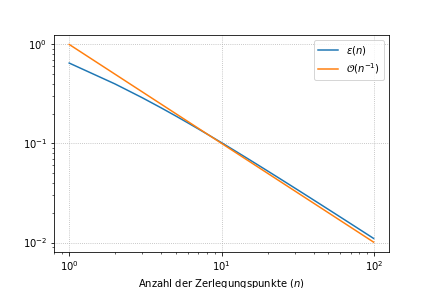
\includegraphics
  [width = 0.5 \textwidth]
  {Fehler zum Endzeitpunkt vs. Anzahl der Zerlegungspunkte}
  \caption{Konvergenzplot}
  \label{Konvergenzplot}
\end{figure}

\end{solution}

\begin{exercise}

Seien $A, M \in \R^{n \times n}$ symmetrisch, positiv definit und $f \in C([0, T], \R^n)$. Weiter sei $y_{y_0} \in C^1([0, T], \R^n)$ Lösung des Anfangswertproblems

\begin{align*}
  M y^\prime(t) = -A y(t) + f(t),
  \quad
  t \in [0, T],
  \quad
  y(0) = y_0
\end{align*}

zu einem beliebigen $y_0 \in \R^n$.
Zeigen Sie elementar, dass $y_0 \mapsto y_{y_0}(t)$ für jedes $t \in [0, T]$ Lipschitzstetig mit Lipschitz-Konstante $1$ bezüglich der von $M$ induzierten Norm $\norm[M]{\cdot}: x \mapsto \sqrt{x^T M x}$ ist.
Ist das Problem in diesem Sinne gut konditioniert?

\end{exercise}

\begin{solution}

Trivial!

\end{solution}

\begin{exercise}

Sei $y \in C^1(\R_{\geq 0}, \R)$ Lösung des Anfangswertproblems

\begin{align*}
  y^\prime(t) = \lambda y(t),
  \quad
  t > 0,
  \quad
  y(0) = y_0
\end{align*}

mit einem $\lambda < 0$.
Sei $h > 0$ eine konstante Schrittweite, $t_j := jh$, $j \in \N_0$, und $y^e_j$ bzw. $y^i_j$ die Approximationen an $y(t_j)$ aus dem expliziten bzw. impliziten Eulerverfahren.
Untersuchen Sie in Abhängigkeit von $\lambda$ und $h$ das Verhalten von $y^e_j$ bzw. $y^i_j$ für $j \to \infty$ und vergleichen Sie es mit dem der exakten Lösung $y(t_j)$.

\end{exercise}

\begin{solution}

Das Anfangswertproblem kann durch $f(t, y) = \lambda y$ beschrieben werden. Man verifiziert unmittelbar, dass die exakte Lösung folgende ist.

\begin{align*}
  y(t) = e^{\lambda t} y_0
\end{align*}

Damit erhält man

\begin{align*}
  y(t_j) \xrightarrow{j \to \infty} 0.
\end{align*}

Die Approximationen $y_j^{\mathrm{e}}$ und $y_j^{\mathrm{i}}$ sollten also auch für $j \to \infty$ verschwinden. \\

Mit $j \in \N_0$ lautet die explizite Euler Methode

\begin{align*}
  \Phi(t_j, y_j^{\mathrm{e}}, h) := f(t_j, y_j^{\mathrm{e}}),
  \quad
  y_{j+1}^{\mathrm{e}} := y_j^{\mathrm{e}} + h \Phi(t_j, y_j^{\mathrm{e}}, h).
\end{align*}

Man erhält also konkret

\begin{align*}
  y_{j+1}^{\mathrm{e}}
  =
  y_j^{\mathrm{e}} + h \lambda y_j^{\mathrm{e}}
  =
  (1 + h \lambda) y_j^{\mathrm{e}}.
\end{align*}

Damit folgt unmittelbar

\begin{align*}
  y_j^{\mathrm{e}}
  =
  (1 + h \lambda)^j y_0.
\end{align*}

Dieser Ausdruck ist für $y_0 = 0$ offensichtlich konstant $0$ und somit dagegen konvergent.
Er verschwindet aber auch für $|1 + h \lambda| < 1$.
Sollte allerdings $y_0 \neq 0$ und $|1 + h \lambda| \geq 1$ so konvergiert er nicht.
Dabei oszilliert die Approximation um die $t$-Achse, wenn $1 + h \lambda < 0$.
Um das zu vermeiden, muss für gegebenes $\lambda < 0$, $h > 0$ hinreichend klein sein. \\

Mit $j \in \N_0$ lautet die implizite Euler Methode

\begin{align*}
  \Phi(t_j, y_j^{\mathrm{i}}, y_{j+1}^{\mathrm{i}}, h) := f(t_{j+1}, y_{j+1}^{\mathrm{i}}),
  \quad
  y_{j+1}^{\mathrm{i}} := y_j^{\mathrm{i}} + h \Phi(t_j, y_j^{\mathrm{i}}, y_{j+1}^{\mathrm{i}}, h).
\end{align*}

Man erhält also konkret

\begin{align*}
  y_{j+1}^{\mathrm{i}}
  =
  y_j^{\mathrm{i}} + h \lambda y_{j+1}^{\mathrm{i}}
  \Rightarrow
  y_{j+1}^{\mathrm{i}}
  =
  (1 - h \lambda)^{-1} y_j^{\mathrm{i}}.
\end{align*}

Damit folgt unmittelbar

\begin{align*}
  y_j^{\mathrm{i}}
  =
  (1 - h \lambda)^{-j} y_0.
\end{align*}

Dieser Ausdruck ist für $y_0 = 0$ offensichtlich konstant $0$ und somit dagegen konvergent.
Er verschwindet aber auch für

\begin{align*}
  |1 - h \lambda|^{-1} < 1
  \Leftrightarrow
  1 < |1 - \underbrace{h \lambda}_{< 0}| = 1 - h \lambda
  \Leftrightarrow
  h \lambda < 0.
\end{align*}

Wir erkennen also, dass bei diesem Anfangswertproblem die Approximation mit dem impliziten Eulerverfahren vorzuziehen ist, da
diese unter den gegebenen Voraussetzungen für $j \to \infty$ immer verschwindet. \\

Schließlich, konvergieren die Approximationen beider Eulerverfahren, für $h \to 0$, gegen die exakte Lösung.

\begin{align*}
  y_j^{\mathrm{e}}
  =
  \pbraces
  {
    (1 + h \lambda)^\frac{1}{h \lambda}
  }^{\lambda t_j}
  \xrightarrow{h \to 0}
  y(t_j),
  \quad
  y_j^{\mathrm{i}}
  =
  -\pbraces
  {
    (1 - h \lambda)^\frac{1}{h \lambda}
  }^{-\lambda t_j}
  \xrightarrow{h \to 0}
  y(t_j)
\end{align*}

\end{solution}

\begin{exercise}

Beweisen Sie folgende Variation des Satzes 1.3 aus der Vorlesung:
$f$ sei bezüglich des zweiten Argumentes nur einseitig Lipschitz-stetig, d.h. es existiert ein $L_+ \in \R$ mit

\begin{align*}
  \abraces{f(t, y) - f(t, z), y - z}
  \leq
  L_+ \norm[2]{y - z}^2,
  \quad
  (t, y), (t, z) \in J \times \Omega.
\end{align*}

Weiter sei auch $z$ eine Lösung der Differentialgleichung $z^\prime = f(t, z)$ (d.h. $\delta = 0$ in Satz 1.3). Dann gilt

\begin{align*}
  \norm[2]{y(t) - z(t)}
  \leq
  \norm[2]{y(t_0) - z(t_0)} e^{L_+ (t - t_0)},
  \quad
  t \geq t_0.
\end{align*}

\end{exercise}

\begin{solution}

Zuerst, bemerken wir, dass

\begin{align*}
  \frac{d}{d \tau} \norm[2]{y(\tau) - z(\tau)}^2
  & =
  \sum_{i=1}^n \frac{d}{d \tau} (y_i(\tau) - z_i(\tau))^2
  =
  \sum_{i=1}^n 2 (y_i(\tau) - z_i(\tau))(y_i^\prime(\tau) - z_i^\prime(\tau)) \\
  & =
  2 \abraces
  {
    y^\prime(\tau) - z^\prime(\tau),
    y(\tau) - z(\tau)
  }_2
  =
  2 \abraces
  {
    f(\tau, y(\tau)) - f(\tau, z(\tau)),
    y(\tau) - z(\tau)
  }_2
  \leq
  2 L_+ \norm[2]{y(\tau) - z(\tau)}^2.
\end{align*}

Aus dem Hauptsatz der Differnetial- und Integralrechnung, der Dreiecksungleichung, folgt also

\begin{align*}
  \norm[2]{y(t) - z(t)}^2
  & \leq
  \norm[2]{y(t_0) - z(t_0)}^2
  +
  \Int[t_0][t]
  {\frac{d}{d \tau} \norm[2]{y(\tau) - z(\tau)}^2}{\tau} \\
  & \leq
  \norm[2]{y(t_0) - z(t_0)}^2
  +
  2 L_+ \Int[t_0][t]
  {\norm[2]{y(\tau) - z(\tau)}^2}{\tau}.
\end{align*}

Mit dem Grönwall-Lemma, und den (jetzt nicht unmotivierten) Definitionen

\begin{align*}
  v(t) := \norm[2]{y(t) - z(t)}^2,
  \quad
  A := v(t_0),
  \quad
  B := 0,
\end{align*}

erhalten wir

\begin{align*}
  \norm[2]{y(t) - z(t)}^{2}
  \leq
  \norm[2]{y(t_0) - z(t_0)}^2 e^{2 L_+ (t - t_0)}.
\end{align*}

Wenn man hier noch die $\sqrt{\cdot}$ zieht, folgt die Behauptung.

\end{solution}

\begin{exercise}

Sei $A \in \R^{n \times n}$ symmetrisch und $y \in C^1([0, T], \R^n)$ Lösung des Anfangswertproblems

\begin{align*}
  y^\prime(t) = A y(t),
  \quad
  t \in [0, T],
  \quad
  y(0) = y_0.
\end{align*}

Berechnen Sie die Lipschitz-Konstante sowie die einseitige Lipschitz-Konstante der zugehörigen Funktion $f$ und vergleichen Sie die Aussage aus dem Satz 1.3 mit der Aussage aus Aufgabe 4.

Hinweis: Symmetrische Matrizen sind diagonalisierbar.

\end{exercise}

\begin{solution}

Die zugehörige Funktion ist $f: (t, y) \mapsto Ay$.
Also $\Forall (t, y), (t, z) \in \R \times \R^n:$

\begin{align*}
  \norm{f(t, y) - f(t, z)}
  =
  \norm{A (y - z)}
  \leq
  \norm{A} \cdot \norm{y - z}.
\end{align*}

Damit ist die Lipschitz-Konstante $L = \norm{A}$. \\

Weil $A$ diagonalisierbar ist, existiert eine Basis $B \in \R^{n \times n}$ aus Eigenvektoren von $A$, sodass $D := B^{-1} A B$ eine Diagonalmatrix ist.
$\rho(A) := \max \Bbraces{|\lambda|: \lambda \text{ Eigenwert von } A}$ ist der Spektralradius von $A$.
Weil $A = A^T$ symmetrisch ist, folgt $\Forall (t, y), (t, z) \in \R \times \R^n:$

\begin{align*}
  \abraces{f(t, y) - f(t, z), y - z}
  & =
  \abraces{A (y - z), y - z}
  =
  (y - z)^T A (y - z)
  =
  (y - z)^T B D B^{-1} (y - z) \\
  & \leq
  (y - z)^T B \rho(A) B^{-1} (y - z)
  =
  \rho(A) (y - z)^T (y - z)
  =
  \rho(A) \norm[2]{y - z}^2.
\end{align*}

Damit ist die einseitige Lipschitz-Konstante $L_+ = \rho(A)$. \\

Für jede natürliche Matrixnorm $\norm{\cdot}$ und jede Matrix $A \in \K^{n \times n}$, gilt $\rho(A) \leq \norm{A}$. Also ist die einseitige Lipschitz-Konstante \enquote{besser} also die Lipschitz-Konstante, d.h. $L_+ \leq L$. \\

Gemeinsam mit der Aufgabe 4, erhält man also dieselbe Konklusio, wie in Satz 1.3, mit $\delta = 0$, also einer exakten Lösung $z$.

\end{solution}


\end{document}
